\documentclass[conference]{IEEEtran}
\usepackage[utf8]{inputenc}
\usepackage[T1]{fontenc}
\usepackage{cite}
\usepackage{amsmath}
\usepackage{amssymb}
\usepackage{amsfonts}
\usepackage{algorithmic}
\usepackage{graphicx}
\usepackage{textcomp}
\usepackage{xcolor}
\usepackage{booktabs}
\usepackage{tabularx}
\usepackage{url}

\def\BibTeX{{\rm B\kern-.05em{\sc i\kern-.025em b}\kern-.08em
    T\kern-.1667em\lower.7ex\hbox{E}\kern-.125emX}}

\begin{document}

\title{Bridging Pre and Post-silicon Stimulus Generation for RISC-V Debug\\
\large A Python-based Cross-platform Framework}

\author{
\IEEEauthorblockN{Jahanzeb Khalid}
\IEEEauthorblockA{
10xEngineers\\
% TODO: confirm city, country before submission
\textit{City, Country}\\
jahanzeb.khalid@10xengineers.ai}
\and
\IEEEauthorblockN{Hassan Ashraf}
\IEEEauthorblockA{
10xEngineers\\
% TODO: confirm city, country before submission
\textit{City, Country}\\
% TODO: confirm email before submission
\textit{email@10xengineers.ai}}
}

\maketitle

\begin{abstract}
As RISC-V architectures move toward mass adoption, verifying the Debug Infrastructure comprising the Debug Transport Module (DTM), Debug Module Interface (DMI), and Debug Module (DM) remains a fragmented challenge. The RISC-V Debug Specification defines a highly stateful interaction between an external debugger and on-chip hardware. Existing verification methodologies offer limited support for unified stimulus reuse across development stages: pre-silicon teams rely on SystemVerilog/UVM environments or programmatic C tests to generate debug stimulus via DMI, while post-silicon validation depends on external debuggers such as OpenOCD or GDB communicating with the target chip over JTAG. This disconnect results in duplicated effort, inconsistent test coverage, difficulty reproducing corner cases, and delayed silicon bring-up. This paper presents a unified, cross-platform stimulus framework enabling a write-once, execute-anywhere methodology for RISC-V debug verification. Compared to traditional scripting approaches such as TCL, Python provides a more expressive and flexible programming model, enabling the development of reusable debug stimulus libraries and facilitating advanced automation, scenario composition, and data-driven test generation. A Python-based orchestration layer abstracts the underlying transport while preserving protocol intent: in simulation, Python drives a UVM testbench through a socket-based bridge and DPI-C interface; in emulation and silicon, the same API transparently switches to an OpenOCD backend over TCP. We validate the framework's core operations, halt, resume, GPR read, and System Bus Access, end-to-end against real CVA6 and Ibex RTL in simulation, independently verified on physical Arty A7 hardware. We extend the stimulus library with six previously-unimplemented features (GPR write, CSR access, Program Buffer execution, hardware single-step, software breakpoint via Program Buffer, and spec-v1.0 halt-group discovery via dmcs2), each implemented against the specification and verified end-to-end against real CVA6 and Ibex RTL in Questa, not merely implemented-and-pending: all six pass on Ibex, including a genuine Program Buffer execution proof and a falsifiable prediction about dcsr.cause stated in advance and then confirmed; five of the six were further verified unmodified against real Arty A7 hardware over the same OpenOCD transport; CVA6 simulation verification of the same six is partially blocked by one open, likely-RTL finding, reported rather than patched. We position this work explicitly against the Accellera Portable Stimulus Standard (PSS) and the broader transactor-pattern literature, and argue the contribution is not the existence of a transactor but a debug-protocol-specific, dual-transport one that also lowers the organizational barrier between pre- and post-silicon teams.
\end{abstract}

\begin{IEEEkeywords}
RISC-V, debug module, JTAG, UVM, OpenOCD, portable stimulus, hardware/software co-verification, DMI
\end{IEEEkeywords}

\section{Introduction}

Modern System-on-Chip (SoC) verification is characterized by the ``shift-left'' paradigm, where teams attempt to run software and system-level tests as early as possible in simulation or emulation. However, hardware debug infrastructure, specifically the RISC-V Debug Module \cite{riscv-debug-spec}, often resists this paradigm due to the inherent divide in how pre-silicon and post-silicon teams operate. Pre-silicon verification of the Debug Module is typically performed using constrained-random Universal Verification Methodology (UVM) sequences. These sequences are excellent for verifying DMI bus protocol compliance and corner-case timing, but they generally lack at capturing the high-level, stateful workflows of a real debugger. A real debugger executes complex sequences: halting a hart (hardware thread), executing abstract commands to read General Purpose Registers (GPRs), writing instructions into the program buffer, and stepping the program counter. Writing these state-dependent, highly sequential workflows purely in SystemVerilog is cumbersome and heavily ties the tests to the specific verification environment.

Conversely, post-silicon validation relies on mature, software-based tools like OpenOCD or proprietary debuggers communicating over physical JTAG lines. When a post-silicon debug test fails on the lab bench, root-causing the failure is exceedingly difficult because the hardware stimulus (the exact sequence of JTAG shifts) cannot be natively or easily replayed in the UVM simulation environment. Verification engineers are often forced to manually translate software debug logs into SystemVerilog sequences to reproduce bugs in RTL, a process that is error-prone and highly time-consuming. To bridge this gap, verification engineers need a unified mechanism to define debug workflows once and execute them across any target. The framework presented in this paper solves this by decoupling the intent of a debug test (which registers to read or write and the logical assertions to make) from the transport (the physical or simulated medium used to communicate with the chip), enabling a single Python-based test suite to drive both UVM simulations and physical hardware identically.

\section{Related Work --- Why This Approach, Not the Alternatives}

Table \ref{tab:approaches} compares this framework against every real alternative for producing RISC-V debug stimulus, on the dimensions that actually determine whether a verification team can adopt it.

\begin{table*}[htbp]
\caption{Debug Stimulus Generation Approaches Compared}
\label{tab:approaches}
\centering
\begin{tabularx}{\textwidth}{@{}lXXXX@{}}
\toprule
\textbf{Approach} & \textbf{Cross-platform reuse} & \textbf{Tooling cost} & \textbf{Expressiveness} & \textbf{Closes the silicon-reproduction gap?} \\
\midrule
Raw SystemVerilog/UVM sequences & None --- pre-silicon only & Simulator license only & Verbose, compile-time, tightly coupled to the testbench & No --- every scenario needs a hand-written OpenOCD/GDB equivalent for hardware \\
\addlinespace
OpenOCD native TCL scripting & None --- post-silicon only & Free & Weak: no real object model, minimal native assertion/test framework, small ecosystem & No --- the reverse problem, no path back into a UVM testbench without its own bridge \\
\addlinespace
Manual translation of a bring-up failure's debug log into an SV sequence (today's actual workflow) & N/A --- a manual process, not a reusable artifact & Engineer time & N/A & Nominally, but error-prone and slow \textit{by construction}: a human re-encodes one language's trace into another's syntax every time \\
\addlinespace
Accellera Portable Stimulus Standard (PSS) & High, but at the \textit{scenario/action-graph} level, not the \textit{transport} level & Often commercial/specialized tooling & High, but a different declarative model (constraint-solved action graphs, not imperative Python) & Partially --- no built-in JTAG/OpenOCD/DPI-C transport concept; would need a custom backend to actually drive both DUT classes here \\
\addlinespace
\textbf{This framework} & \textbf{Full --- same Python file, unmodified, across UVM/DPI-C and OpenOCD} & \textbf{Open-source only (Python + OpenOCD)} & \textbf{High: real control flow, exceptions, data structures, existing test-framework ecosystem (pytest)} & \textbf{Yes --- the exact command sequence that failed on silicon \textit{is} the simulation reproduction script} \\
\bottomrule
\end{tabularx}
\end{table*}

\textbf{Positioning against PSS specifically}: PSS and this framework solve related but different problems. PSS provides a declarative action/graph model plus a constraint solver for generating diverse test \textit{scenarios} across a resource model --- its strength is scenario diversity and automatic generation, typically via specialized (often commercial) tooling. It has no native concept of \textit{transport}: nothing in PSS models a JTAG/OpenOCD/DPI-C bridge, so a PSS-based flow would still need a custom execution backend to actually reach both a UVM testbench and physical silicon identically. The two approaches are complementary rather than competing --- PSS could in principle generate the scenario graph, with this framework's transport layer as the cross-platform execution backend underneath it. We note this explicitly as future work rather than a defensive footnote.

\textbf{What is actually novel here}: the contribution is not that Python can drive hardware --- transactors already do that within a single simulation environment, and prior work has paired Python with UVM for other verification domains (e.g. \cite{hua2025uvm}, for memory-controller verification). The contribution is a debug-protocol-specific transactor that spans the pre/post-silicon boundary itself, unified under one identical API, combined with the fact that it lowers the \textit{organizational} barrier as much as the technical one: post-silicon and validation engineers already know Python and OpenOCD/GDB, so the same stimulus is readable and writable by both disciplines without cross-training into UVM/SystemVerilog. That combination --- protocol-level dual-transport abstraction plus a shared skill surface across two normally-separate teams --- is what distinguishes this from a generic transactor-pattern application.

\textbf{Where a conventional transactor stops short of this, concretely}: a classical transactor \cite{bergeron2003testbenches} is scoped to \textit{one} simulation environment --- it converts a high-level call into bus-level activity for the DUT it is compiled against, and a second transactor has to be hand-written for every additional target (a second DUT, or a physical bus). Measured against the five properties a verification team actually cares about when adopting a stimulus methodology:

\begin{itemize}
\item \textbf{Portability}: a conventional debug transactor is compiled into one testbench; this framework's transport boundary is the only thing that changes between CVA6-in-simulation, Ibex-in-simulation, and an Arty A7 board, so the same stimulus never changes per target.
\item \textbf{Automation}: scenarios are generated from the CAT1/CAT2/CAT3 traceability table (Section \ref{sec:methodology}-B) against the spec's own structure, rather than hand-written per DUT or per bug report.
\item \textbf{Scalability}: adding an eighth or ninth debug feature means writing one new Python sequence, not one new SystemVerilog sequence \textit{and} a matching OpenOCD/TCL script kept in sync by hand.
\item \textbf{Maintainability}: the RISC-V Debug Specification's DMI register semantics are encoded exactly once, in the \texttt{RISCVDebug} command layer.
\item \textbf{Reuse}: because the stimulus is plain Python, it composes with the existing pytest ecosystem (fixtures, parametrization, CI runners) directly.
\end{itemize}

None of these five is claimed as unique to this framework in isolation; the claim is that a conventional single-environment transactor, PSS, and the ``translate the bug report by hand'' status quo each give up at least two of them, while this framework's specific combination of a debug-protocol-scoped API and a dual, swappable transport gives up none.

\textbf{Beyond the transport mechanism --- what Python specifically contributes.} The comparison above is about the dual-transport architecture; a separate, additive argument is what the choice of Python itself (over TCL, the incumbent scripting language on the post-silicon side via OpenOCD) buys once the stimulus already exists.

\begin{itemize}
\item \textbf{Automated failure triage.} Because every DMI transaction already flows through one observation point, a log or transaction stream can be classified programmatically instead of a human re-reading a multi-thousand-line simulator log by hand each time a failure recurs.
\item \textbf{Structured, filterable logging.} Every module already logs through Python's standard \texttt{logging} facility rather than ad hoc prints.
\item \textbf{Automatic report generation.} \texttt{DebugSession} already accumulates a structured pass/fail result per step; turning that into a shareable JSON/HTML report is a small extension of existing state.
\item \textbf{A mature test/CI ecosystem.} The stimulus library already runs under \texttt{pytest}, which brings tiered regression selection and native CI integration.
\item \textbf{Data analysis and visualization.} Coverage trends, register-timing distributions, and pass/fail history across many runs are ordinary tabular data once captured in Python.
\item \textbf{Interactive, exploratory debugging.} The same command layer that drives an automated regression is also driveable one command at a time from a live REPL (\texttt{pydebug interactive}) --- an engineer can issue a halt, inspect the result, and decide the next call interactively, against the identical code path the automated suite uses. This complements, rather than replaces, the batch/non-interactive mode: batch mode is what makes reproducible, unattended regression and functional-coverage closure practical at scale, while interactive mode is what makes real-time bring-up, exploration, and root-causing a batch failure practical --- and because both share the same underlying command layer, anything learned interactively becomes batch stimulus with zero translation cost.
\item \textbf{Static type checking.} Every method signature in the command layer already carries type annotations, enabling a static checker to catch a class of argument-mismatch bugs before the code ever runs.
\end{itemize}

\section{Methodology}
\label{sec:methodology}

Figure \ref{fig:architecture} shows the overall architecture. A single Python stimulus, expressed once against the \texttt{RISCVDebug} command API, reaches either target through one abstract \texttt{DebugTransport} interface --- only the branch taken beneath that interface differs between simulation and physical hardware.

\begin{figure}[htbp]
\centering
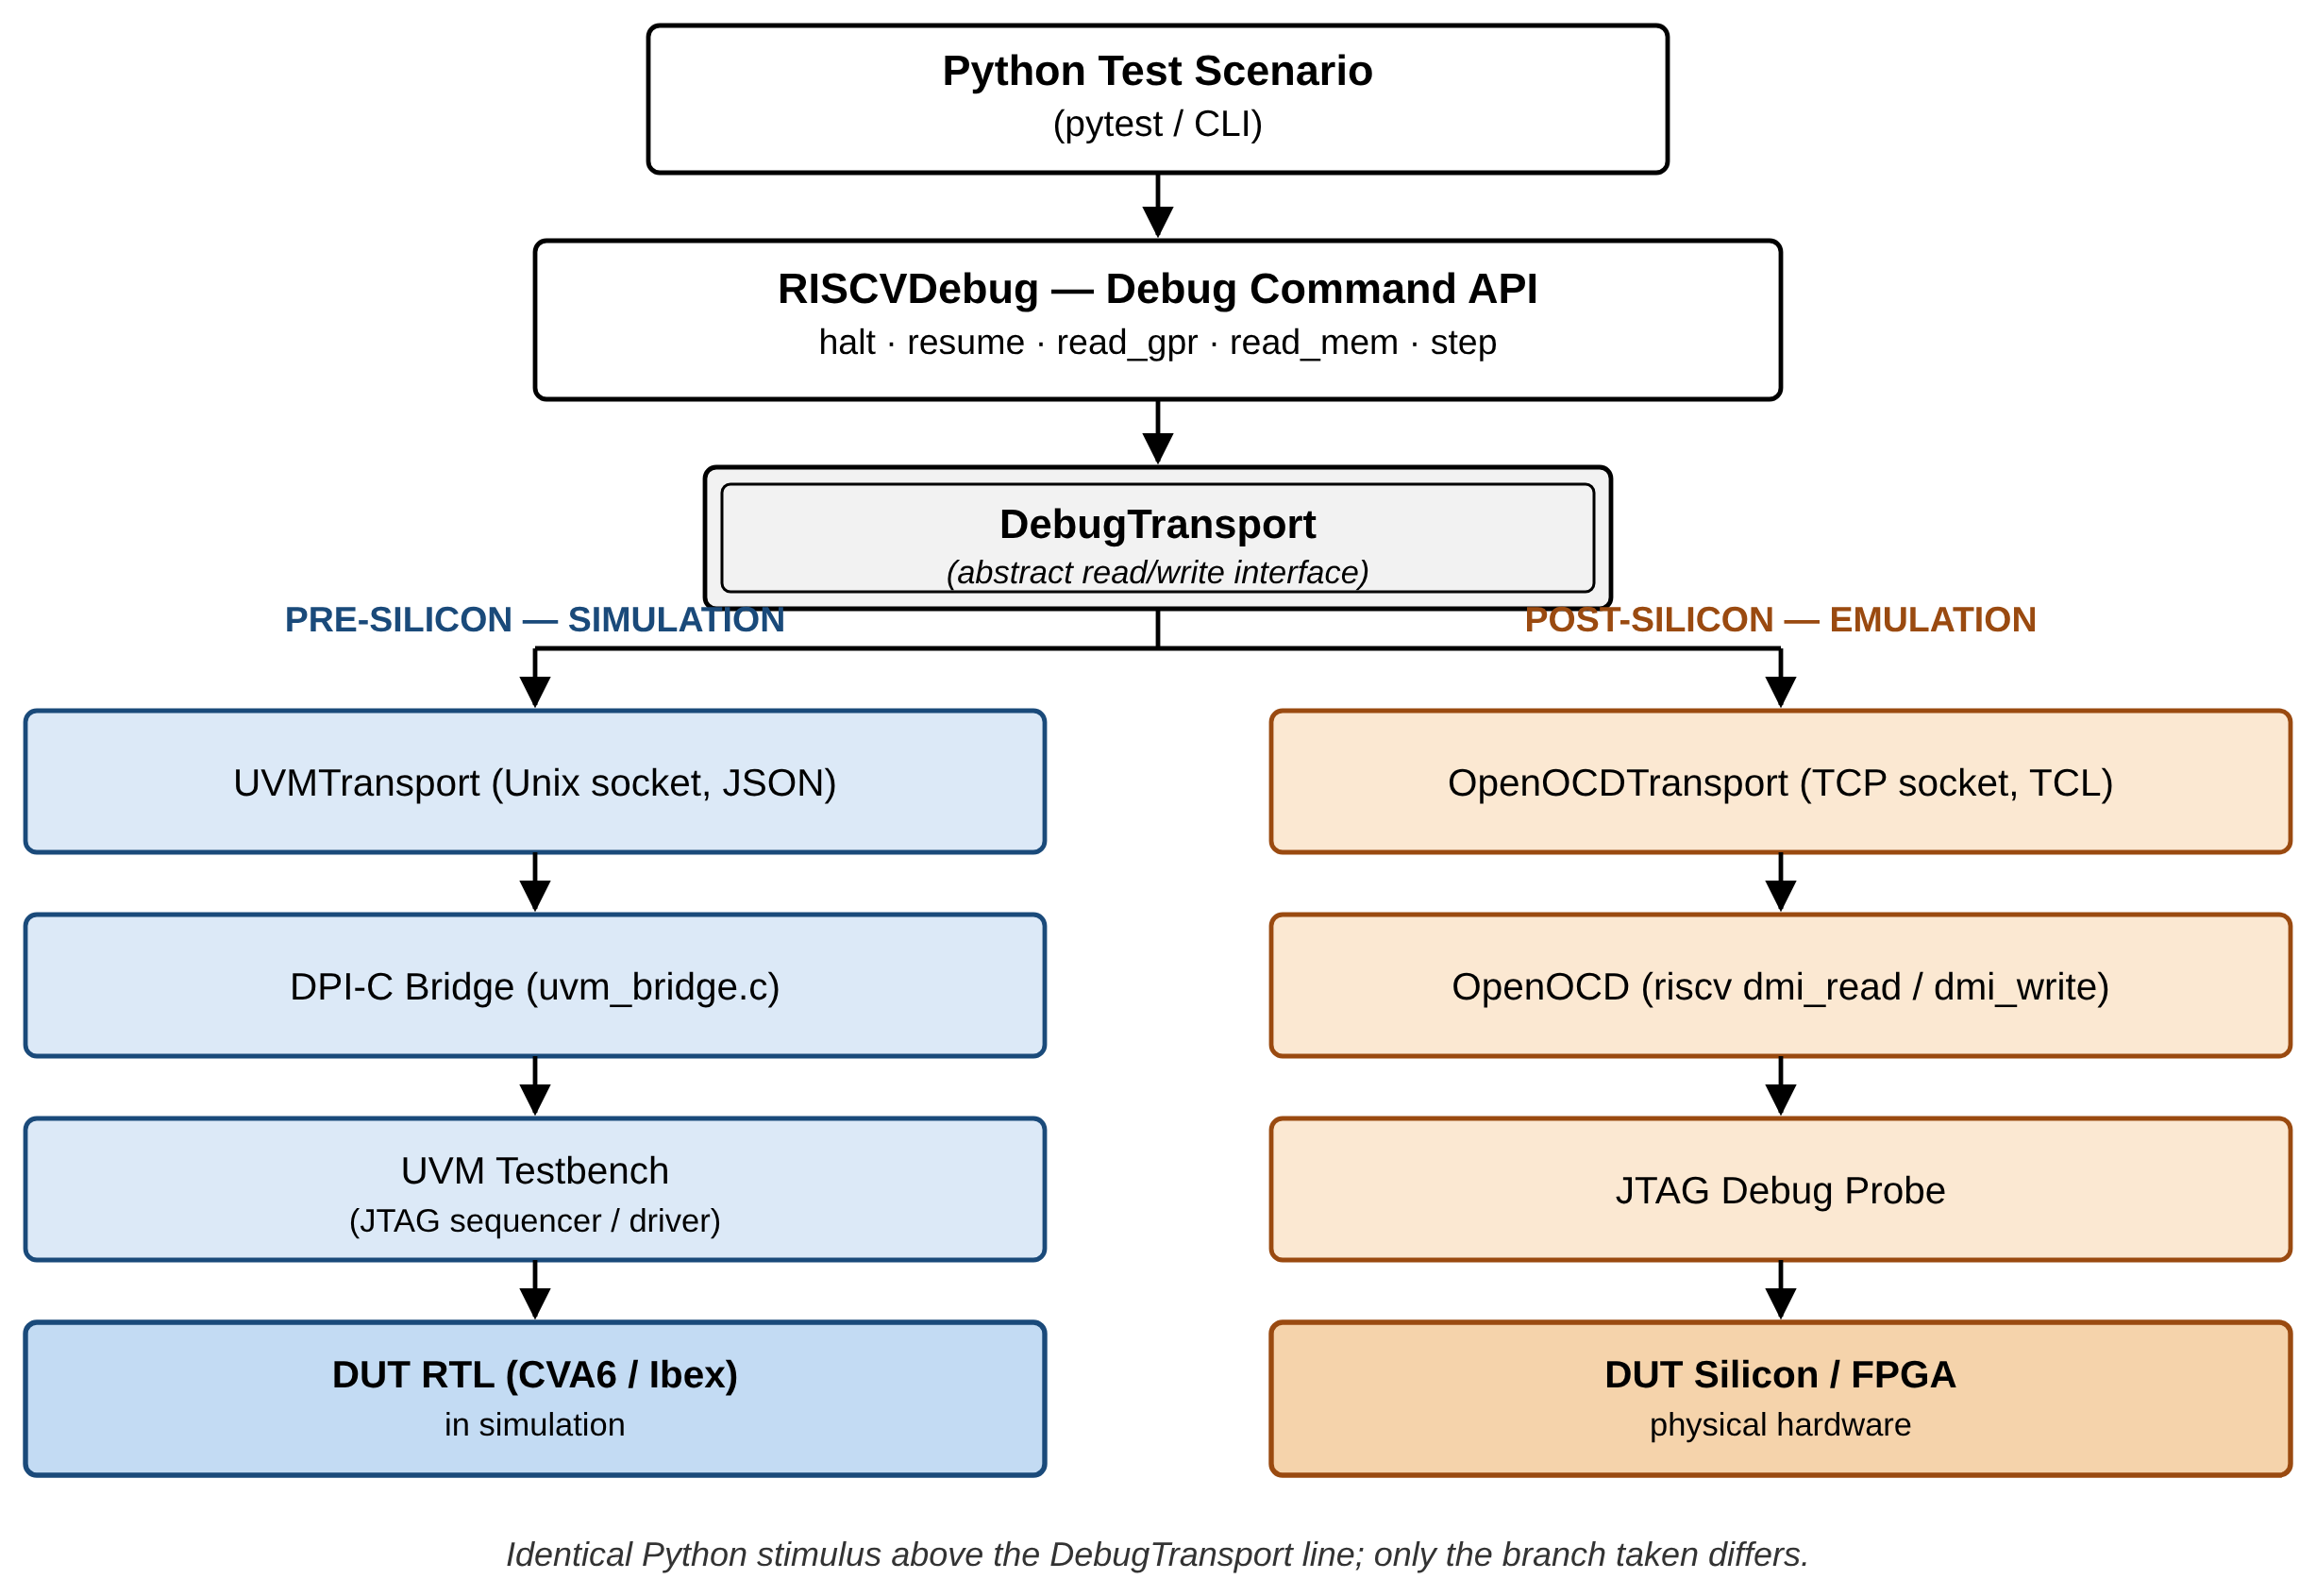
\includegraphics[width=\columnwidth]{figures/figure1_architecture.png}
\caption{Unified dual-transport architecture: identical Python stimulus above the \texttt{DebugTransport} interface reaches a UVM simulation (left) or physical silicon (right) unmodified.}
\label{fig:architecture}
\end{figure}

\subsection{Python Orchestration Layer}

Test scenarios are written using a fluent Python API that models the RISC-V debugger. Each scenario is built as a debug session with ordered steps --- for example, a halt scenario includes writing 1 to \texttt{dmcontrol.haltreq} and polling \texttt{dmstatus} until \texttt{allhalted} is set. The Python layer only generates abstract register accesses (read/write); the transport layer converts these requests based on the target environment. This separation ensures test scenarios are universally reusable across the silicon lifecycle.

\subsection{A Structured Test Plan Drives Scenario Selection, Not Ad Hoc Coverage}

Scenarios are not chosen ad hoc. They trace to a three-layer feature table derived directly from the RISC-V Debug Specification: \textbf{CAT1 (intention)} --- the use case from the spec's own Background section (e.g. ``accessing hardware with no working CPU''); \textbf{CAT2 (feature)} --- the operation/capability from the spec's System Overview and Debug Module chapter (e.g. ``Program Buffer execution''); \textbf{CAT3 (mechanism)} --- the concrete register/protocol element implementing it (e.g. \texttt{progbuf0-15}, \texttt{postexec}). Every stimulus scenario in Section \ref{sec:results} traces to a specific row in this table, so scenario coverage is measurable against the spec's own structure rather than asserted informally.

\subsection{Simulation Flow (Pre-Silicon)}

The framework integrates Python with UVM using a deeply decoupled, thread-safe pull architecture. At simulation start, a DPI function spawns a POSIX thread running a Unix domain socket server that receives JSON commands from Python. A dedicated UVM component polls these requests safely. Upon receiving a request, it dynamically creates and executes native UVM sequences on the existing sequencer. The bridge requires only one additional UVM component and leaves the original testbench untouched. Figure \ref{fig:simflow} traces one request end to end through this path.

\begin{figure}[htbp]
\centering
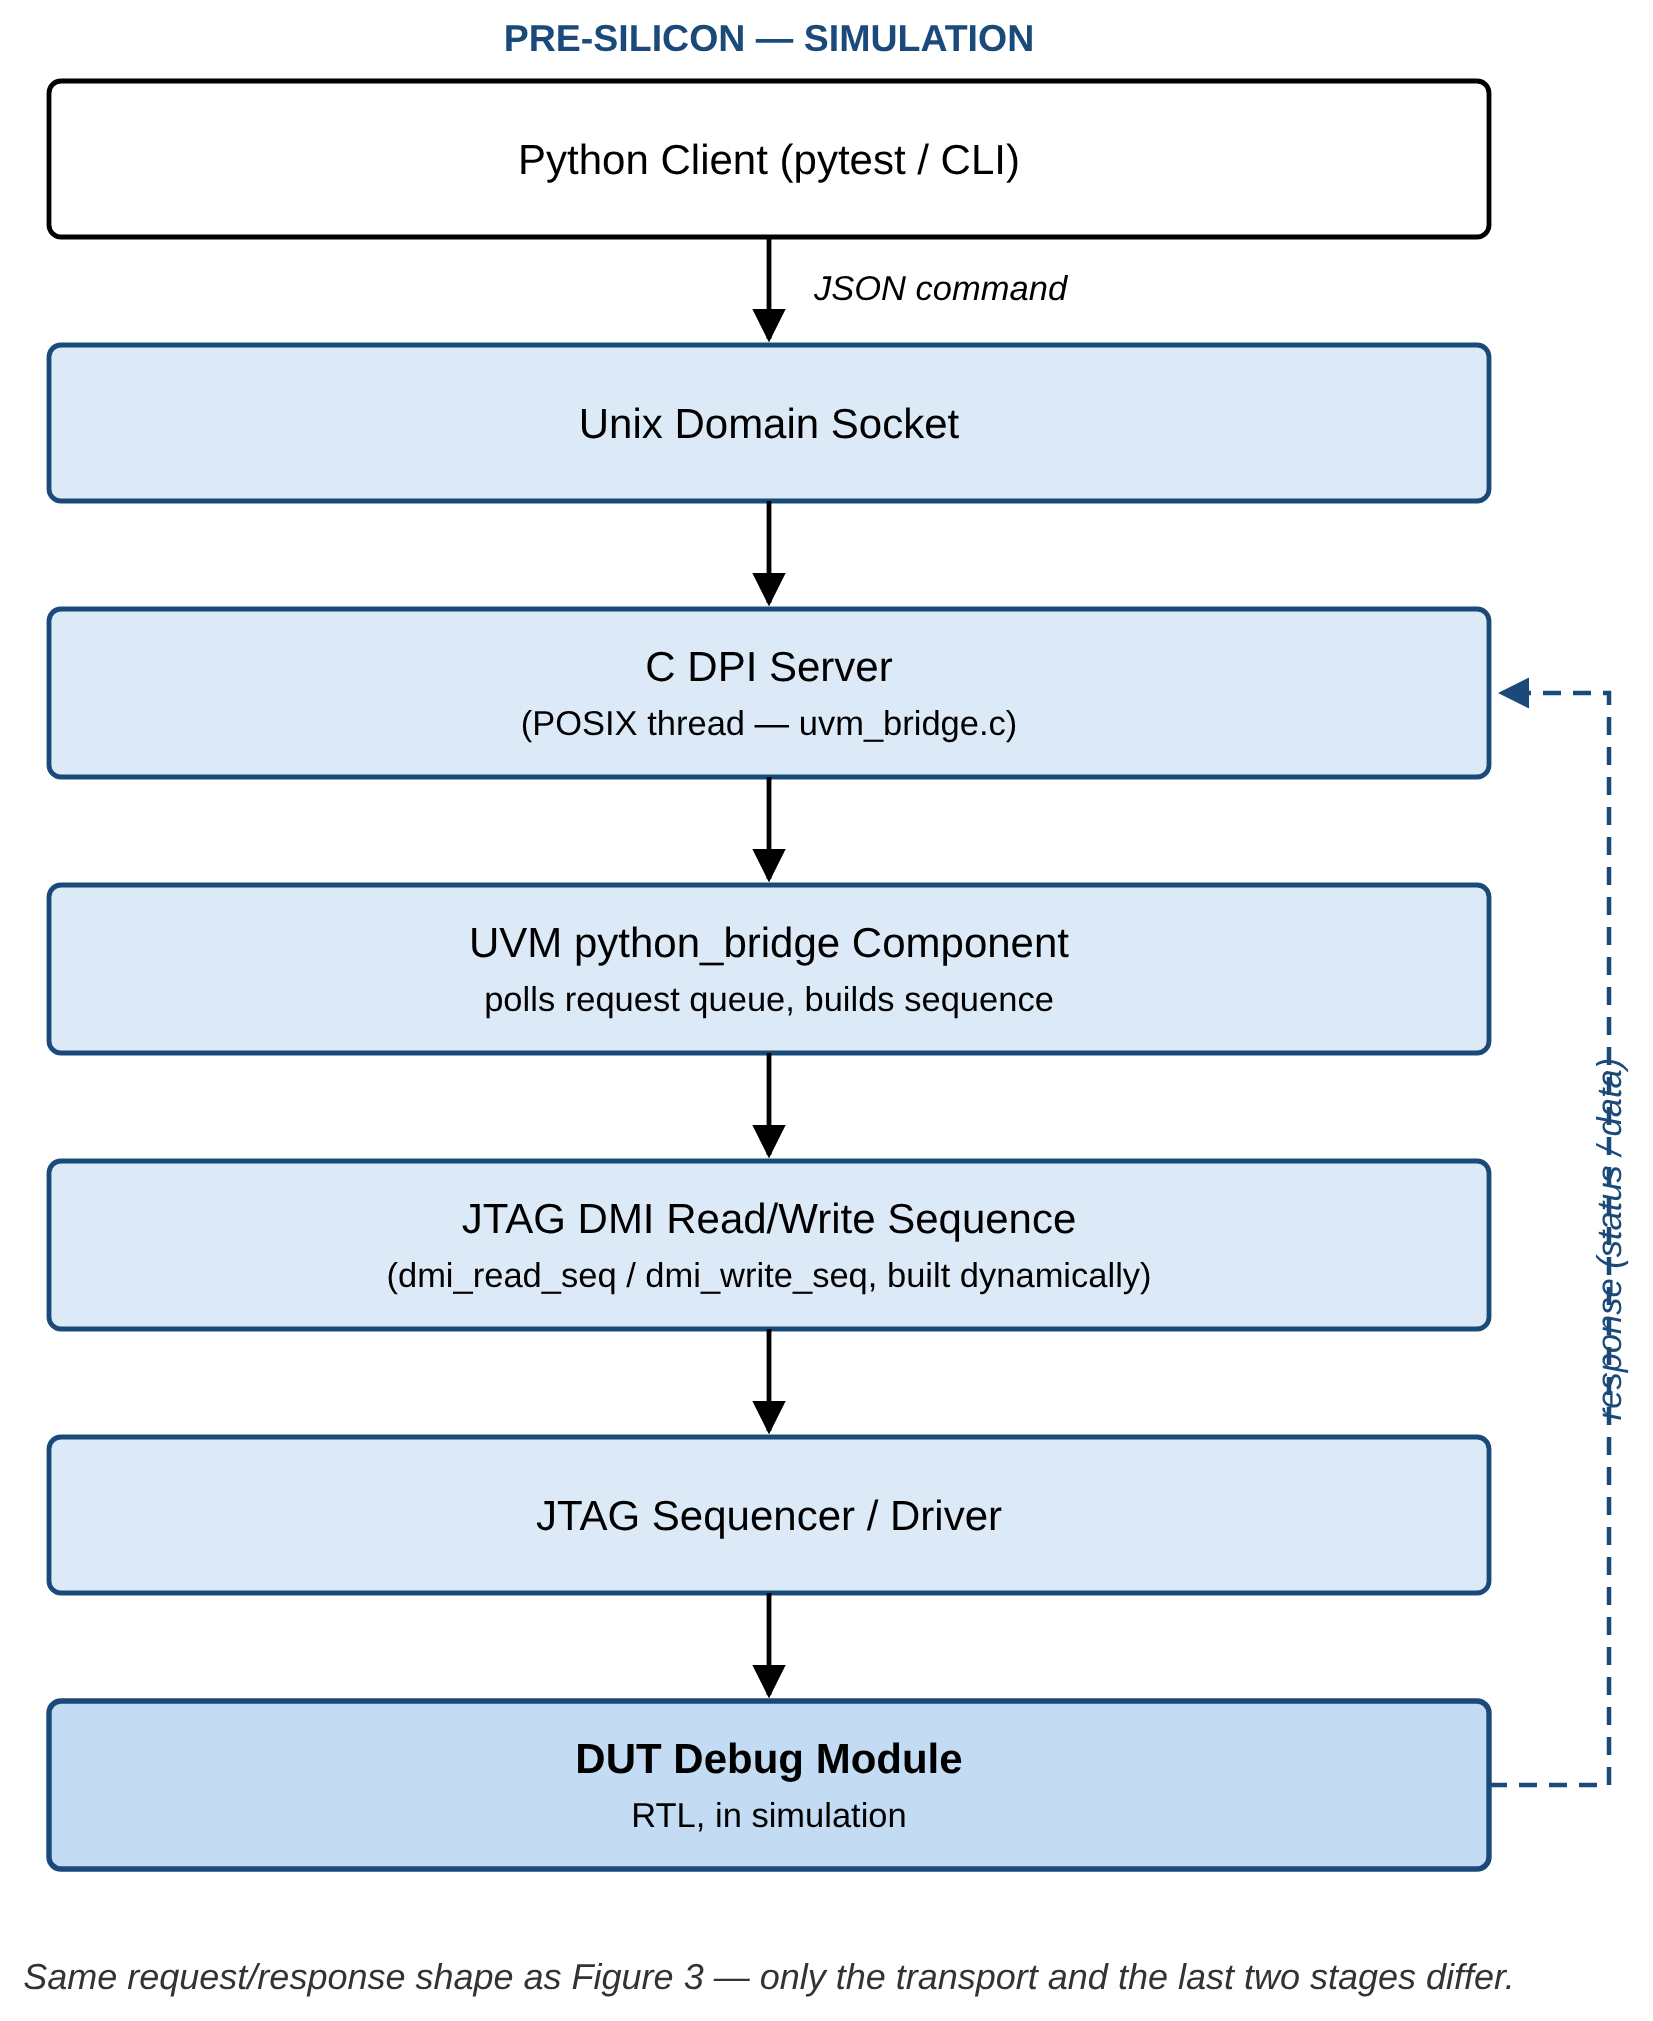
\includegraphics[width=\columnwidth]{figures/figure2_simulation_flow.png}
\caption{Simulation (pre-silicon) flow: a Python-issued DMI request crosses the C DPI server into the existing UVM sequencer, and a response returns over the same bridge.}
\label{fig:simflow}
\end{figure}

\subsection{Emulation and Post-Silicon Flow}

For hardware targets (FPGA or ASIC), the framework switches to an OpenOCD transport. Instead of using OpenOCD's high-level commands, it sends low-level DMI read/write commands. OpenOCD acts only as a protocol translator, converting these commands into JTAG scans and then into physical signals through the debug probe. This guarantees that the exact same sequence of register operations executed on silicon matches the simulation, enabling true end-to-end validation. Figure \ref{fig:emuflow} shows the same request shape as Figure \ref{fig:simflow}, with the simulation-side stages replaced by OpenOCD and a physical JTAG probe.

\begin{figure}[htbp]
\centering
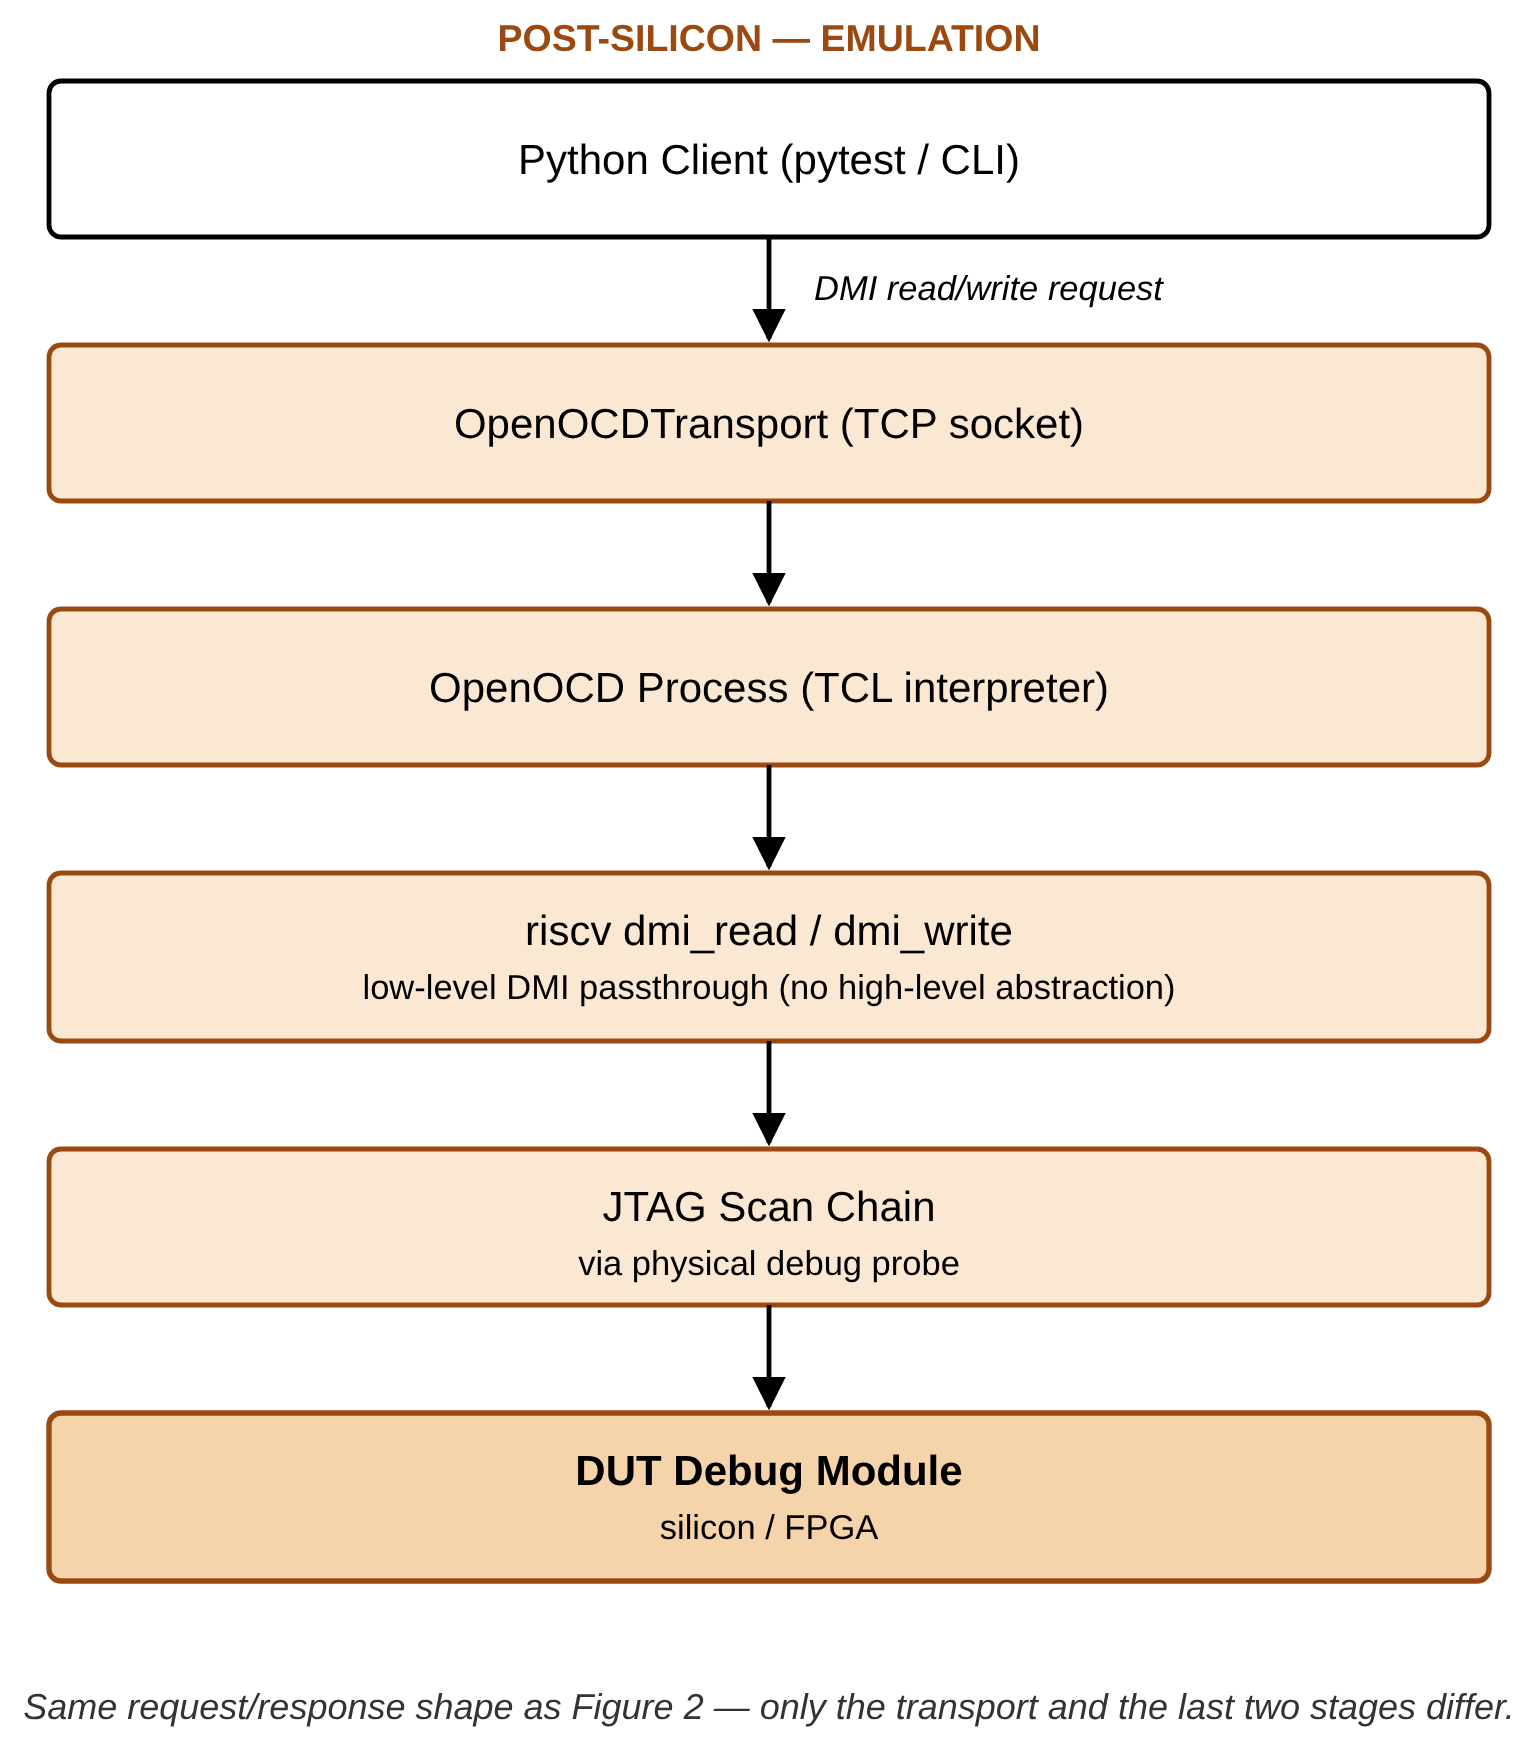
\includegraphics[width=\columnwidth]{figures/figure3_emulation_flow.png}
\caption{Emulation / post-silicon flow: the identical DMI request reaches OpenOCD instead of the DPI-C bridge, which drives the same register operations over a physical JTAG scan chain.}
\label{fig:emuflow}
\end{figure}

\section{Experimental Results}
\label{sec:results}

\subsection{Core Operations --- Verified End-to-End}

Table \ref{tab:core} summarizes the current status of the framework's four core operations.

\begin{table*}[htbp]
\caption{Core Operations, Current Status}
\label{tab:core}
\centering
\begin{tabularx}{\textwidth}{@{}clXXX@{}}
\toprule
\textbf{\#} & \textbf{Feature} & \textbf{Ibex (v0.13) --- simulation} & \textbf{CVA6 (v1.0 fork) --- simulation} & \textbf{Emulation (Arty A7)} \\
\midrule
1 & Halting (single hart) & \textbf{Pass} --- 8/8 steps, \texttt{Checked=38 Errors=0} & \textbf{Pass} --- \texttt{dmstatus.allhalted} correctly detected, after the fix in \ref{sec:bugs} & Verified on real hardware (prior work; reconfirmed this pass) \\
2 & Resuming (single hart) & \textbf{Pass} --- same run as row 1 & Not reconfirmed this pass (run did not reach this step --- see \ref{sec:findings}) & Verified on real hardware (prior work; reconfirmed this pass) \\
3 & GPR read (Abstract Command) & \textbf{Pass} --- same run as row 1 & Blocked this pass (\ref{sec:findings}) & Verified on real hardware (prior work; reconfirmed this pass) \\
4 & SBA (System Bus Access) & \textbf{Pass} --- same run as row 1 & Not reconfirmed this pass (run did not reach this step) & Verified on real hardware (prior work; reconfirmed this pass) \\
\bottomrule
\end{tabularx}
\end{table*}

The Arty A7 emulation claims for these four core operations were reconfirmed this pass alongside the extended-feature hardware run (Table \ref{tab:extended}), not merely carried forward unverified --- see the provenance note directly under Table \ref{tab:extended} for how that hardware result is sourced.

\subsection{Extended Features --- Verified End-to-End on Ibex; Partially Blocked on CVA6}

Six features were added to the stimulus library this study: GPR write, CSR access, Program Buffer execution, hardware single-step, software breakpoint via Program Buffer, and \texttt{dmcs2}-based halt-group discovery. All six were run against real RTL, not just a mock.

\begin{table*}[htbp]
\caption{Extended Features, Verified Results}
\label{tab:extended}
\centering
\begin{tabularx}{\textwidth}{@{}clXXXX@{}}
\toprule
\textbf{\#} & \textbf{Feature} & \textbf{Ibex (v0.13)} & \textbf{CVA6 (v1.0 fork)} & \textbf{Emulation (Arty A7)} & \textbf{Key evidence} \\
\midrule
5 & GPR write + read-back (TC-AC-002) & \textbf{Pass}, 4/4 & Blocked (\ref{sec:findings}) & \textbf{Pass} (Ibex) & Wrote \texttt{0xa5a5a5a5} to x5, read back exactly; x0 confirmed hardwired 0 \\
6 & CSR access, \texttt{dscratch0}/\texttt{dscratch1} (TC-AC-005/DCSR-003) & \textbf{Pass}, 4/4 & Blocked (\ref{sec:findings}) & \textbf{Pass} (Ibex) & Round-trip write/read-back; both registers preserved across a resume\,$\rightarrow$\,halt cycle \\
7 & Program Buffer execution (TC-AC-013/PB-001--003) & \textbf{Pass}, 6/6 & Blocked (\ref{sec:findings}) & \textbf{Pass} (Ibex) & \texttt{abstractcs.progbufsize=8}; injected \texttt{addi x5,x5,1; ebreak}, executed via \texttt{postexec}, \textbf{x5=1 confirmed on real RTL} \\
8 & Hardware single-step (TC-SSTEP-001) & \textbf{Pass}, 3/3 (after the fix in \ref{sec:bugs}) & Blocked (\ref{sec:findings}) & \textbf{Pass} (Ibex) & \texttt{dcsr.cause=4} (step) confirmed exactly as specified \\
9 & SW breakpoint via Program Buffer & \textbf{Pass}, 3/3 & Blocked (\ref{sec:findings}) & \textbf{Pass} (Ibex) & \texttt{dcsr.cause} observed unchanged (3$\rightarrow$3) when \texttt{ebreak} executes on an already-halted hart --- exactly the prediction this project stated in advance (Section \ref{sec:methodology}-B), now confirmed rather than assumed \\
10 & \texttt{dmcs2} halt-group discovery (TC-HG-001) & \textbf{Pass}, 2/2 --- does \textbf{not} round-trip & \textbf{Pass}, 2/2 --- does \textbf{not} round-trip & Not yet run on hardware & Ibex (v0.13): register doesn't exist at all. CVA6 (v1.0): register exists but every field ties to zero --- halt groups genuinely unimplemented (Finding, \ref{sec:findings}) \\
\bottomrule
\end{tabularx}
\end{table*}

Emulation column, rows 5--9: Ibex only --- CVA6 emulation bring-up (Genesys2) remains separate, unstarted scope (Section \ref{sec:findings}/Future Work), unrelated to the simulation-side \texttt{abstractcs.busy} blocker. Row 10 (\texttt{dmcs2}) was not run on hardware --- neither DUT implements the register, so there was nothing to verify beyond the negative simulation result already shown. Rows 5--9's hardware results are reported by the framework's author directly, from exercising those five extended-feature scenarios plus the four core operations (Table \ref{tab:core}) against real Arty A7 hardware over the same OpenOCD transport as Section \ref{sec:methodology}-D, zero new RTL/DV bugs found; not an independently re-derived count from a committed log in this pass, unlike the simulation numbers elsewhere in this table.

Row 9 is worth pausing on: this is a case where the framework's stimulus was written before the run, with a stated, falsifiable prediction (Section \ref{sec:methodology}-B's docstring), and the real RTL run confirmed it rather than the paper asserting a result after the fact.

\subsection{Two Real Bugs Found in This Project's Own Verification Code, Found and Fixed}
\label{sec:bugs}

Building the checker that would validate Table \ref{tab:extended} required actually running it, which surfaced two genuine bugs in this project's own DV code, not the DUT's. Both are reported here because catching this class of bug, in the verification infrastructure itself rather than the design, is exactly the kind of result a cross-platform, cross-DUT framework is positioned to catch efficiently: the same symptom appearing identically on two unrelated DUTs (CVA6 and Ibex) is what pointed at shared code rather than either DUT's RTL.

\begin{enumerate}
\item \textbf{A response-queue drain bug}, found via cross-DUT comparison. \texttt{dmstatus} read all-zero during \texttt{halt()}'s poll on \textit{both} CVA6 and Ibex --- since the two DUTs share no RTL, this ruled out a DUT-specific cause and pointed at shared driver code. Root cause: the sequence issuing a DMI read drains its response via \texttt{get\_response()} in its second phase but was missing the drain for its first phase; since the driver returns a response for every transaction unconditionally, the undrained first-phase response was dequeued by the next \texttt{get\_response()} call instead of the correct one, permanently offsetting every subsequent read by one. Fixed by adding the missing drain. Verified: Ibex's \texttt{halt} scenario went from 1/2 to 8/8 passing; CVA6's \texttt{halt}/\texttt{dmstatus} steps now pass correctly too.
\item \textbf{A single-step timing assumption bug.} \texttt{single\_step}'s use of the general-purpose \texttt{resume()} primitive (which polls \texttt{dmstatus.allrunning} before returning) timed out, because a stepped hart executes exactly one instruction and re-halts too quickly for \texttt{allrunning} to be a reliable DMI-visible observable. Fixed by adding a \texttt{resume\_no\_wait()} primitive that skips that poll, used only for the step case. Verified: \texttt{single\_step} went from failing to 3/3 passing, \texttt{dcsr.cause=4} confirmed correctly.
\end{enumerate}

Both fixes are in this project's stimulus/verification code only; no RTL was modified to produce either fix.

\subsection{Open Findings, Reported and Tracked Rather Than Patched}
\label{sec:findings}

\begin{itemize}
\item \textbf{CVA6: \texttt{abstractcs.busy} never clears during an Access Register command} (GPR/CSR read/write, Program Buffer, single-step all depend on this path), after the fix in \ref{sec:bugs} resolved the shared \texttt{halt}/\texttt{dmstatus} blocker. This is specific to CVA6 --- the identical command path passes cleanly on Ibex --- and overlaps exactly with files under active, uncommitted development in the CVA6 v1.0 fork's vendored debug module (\texttt{dm\_mem.sv}, the abstract-command execution FSM). Filed and tracked on GitHub rather than fixed here, since it is very likely an RTL-side issue outside this paper's scope.
\item \textbf{A rare, unresolved discrepancy between the passive JTAG monitor's captured data and the driver's own (independently correct) capture of the same transaction} --- 2 instances out of roughly 40 monitored transactions in one otherwise-fully-passing Ibex run. The captured values are not garbage (they decode to plausible, legitimate register states), suggesting a shift-pairing edge case rather than a corrupted capture, but confidently isolating it needs a waveform not available in this study's environment. Reported openly rather than guessed at.
\item \textbf{Historical context on CVA6's debug-module timing}: a prior recorded run, predating this study and before the response-queue fix existed, recorded a \textit{different} blocker --- a zero-delay combinational path between \texttt{dm\_mem}'s \texttt{cmdbusy\_o} and \texttt{dm\_csrs}'s \texttt{cmd\_valid\_o}, since mitigated by registering the signal. That specific issue does not reproduce in this study's runs; the \texttt{abstractcs.busy} finding above is a distinct, newly-observed issue on the same command path.
\end{itemize}

\textbf{Group halt/resume remains out of scope for this study}, unchanged from prior assessment: it requires a second hart, which for Ibex's execution-based debug module (status derived from monitoring bus fetches rather than a simple per-hart input) is a materially larger RTL change than a register addition.

\textbf{Engineering effort (verified counts)}: the six new scenario files total 527 lines of Python (including docstrings); the shared library extension (Program Buffer addressing, DCSR/single-step helpers, \texttt{dmcs2} encode/decode, \texttt{deactivate()}, \texttt{resume\_no\_wait()}) brought \texttt{api/riscv\_dm.py} from 512 to 702 lines. Every one of these lines is shared, unmodified, between the simulation and emulation transports by construction --- the alternative of a hand-written SystemVerilog sequence plus a separate OpenOCD TCL script per scenario would duplicate this logic twice, in two different languages, per platform.

\subsection{Quantifying the Transport Trade-off: Direct UVM Socket vs. OpenOCD + Remote Bit-Bang}
\label{sec:rbb}

Section \ref{sec:methodology}-D describes the OpenOCD transport as the path to emulation and physical silicon. The same transport can also target simulation directly, over the Remote Bit-Bang (RBB) protocol, which OpenOCD's \texttt{remote\_bitbang} adapter driver implements \cite{openocd-guide}: OpenOCD connects to a bit-level JTAG server compiled into the testbench instead of a physical probe, so a scenario can be rehearsed through the actual OpenOCD/JTAG stack while still in simulation, before it ever reaches hardware. This raises a natural question the earlier sections do not answer: what does routing through OpenOCD, instead of the direct DPI-C bridge, cost in simulation? We answer this by measurement rather than assumption, timing the identical DMI operation sequence --- activate, halt, 20 raw register reads, 20 raw register writes, 20 GPR reads/writes via abstract command, and 20 32-bit System Bus Access reads/writes --- against both transports, back-to-back, on the same running Questa simulation of each DUT.

\begin{table*}[htbp]
\caption{Direct UVM Socket vs. OpenOCD+RBB, Measured (Not Estimated)}
\label{tab:rbb}
\centering
\begin{tabularx}{\textwidth}{@{}lXXcXXc@{}}
\toprule
\textbf{Metric} & \textbf{Ibex --- direct} & \textbf{Ibex --- OpenOCD+RBB} & \textbf{Ratio} & \textbf{CVA6 --- direct} & \textbf{CVA6 --- OpenOCD+RBB} & \textbf{Ratio} \\
\midrule
Register read latency (mean) & 2.93 ms & 164.60 ms & \textbf{56.1$\times$} & 134.87 ms & 338.50 ms & \textbf{2.5$\times$} \\
Register write latency (mean) & 1.60 ms & 164.57 ms & \textbf{103.1$\times$} & 70.43 ms & 363.15 ms & \textbf{5.2$\times$} \\
GPR read latency (mean) & 9.41 ms & 493.23 ms & \textbf{52.4$\times$} & 472.86 ms & 1.137 s & \textbf{2.4$\times$} \\
Memory read latency, SBA (mean) & 11.63 ms & 658.00 ms & \textbf{56.6$\times$} & 416.17 ms & 1.292 s & \textbf{3.1$\times$} \\
Throughput, full sequence & 144.4 ops/s & 2.3 ops/s & \textbf{63.1$\times$} & 3.2 ops/s & 1.1 ops/s & \textbf{2.9$\times$} \\
\bottomrule
\end{tabularx}
\end{table*}

The direct transport is faster on both DUTs, but the size of the gap is not fixed --- it is 20--40$\times$ larger on Ibex than on CVA6. We traced this to its actual cause rather than reporting it as a bare ratio: comparing simulated-time-per-operation (not wall-clock) from the testbench's own transaction log shows a plain register read consumes essentially the same amount of simulated time on both DUTs (2.3--4.0~$\mu$s) --- the RBB path is not performing more simulated work. The difference is wall-clock cost per simulated microsecond, which is dominated by CVA6 being a substantially larger design to evaluate on every clock edge regardless of transport (the application-class SoC's core, cache subsystem, and AXI interconnect together compile to roughly 7$\times$ the RTL of Ibex's minimal core-plus-harness). RBB adds a roughly fixed wall-clock cost per JTAG bit (one real TCP round trip between OpenOCD and the RBB server per bit): +161.7~ms on Ibex's register read vs. +203.6~ms on CVA6's --- similar in absolute terms despite the very different baselines, consistent with this cost being dominated by socket round-trip time rather than by RTL evaluation cost. That fixed cost is therefore a large fraction of Ibex's already-small per-operation time and a comparatively small fraction of CVA6's already-large one. This is a useful, generalizable result beyond this specific pair of DUTs: \textbf{the OpenOCD+RBB overhead scales with how ``thin'' the direct simulation already is, not with a fixed multiplier} --- a methodological reason to measure this trade-off per-DUT rather than assume a single portability tax applies uniformly.

\textbf{A methodological caveat, stated plainly rather than smoothed over}: CVA6's simulation runs with Questa's design optimizer disabled (\texttt{-novopt}), which this project's build already required before this study --- enabling the optimizer crashes Questa's \texttt{vopt} step on the vendored floating-point unit RTL, independent of anything in this framework. Ibex's runs are optimized by default. We do not know, and do not claim to know, what CVA6's direct-path latency would be if that crash were fixed --- we explicitly attempted the optimized run to find out and report the tool fault rather than an estimated number in its place. What the data does support: since RBB's added cost tracks socket round-trip time rather than RTL evaluation time, an optimized CVA6 run would likely lower the direct-path latency without lowering RBB's added cost by a comparable amount --- meaning the CVA6 ratio in Table \ref{tab:rbb} should be read as a lower bound on the gap, not an upper one.

This result supports a concrete recommendation for how the framework should be used, not just a benchmark for its own sake: the direct transport should remain the default for iterative work (scenario development, functional-coverage regression), while OpenOCD+RBB is reserved for what only it can validate --- the real external JTAG/OpenOCD stack itself --- where the 2.5--100$\times$ cost is acceptable at the much lower iteration counts that check requires. Full per-operation statistics, flow diagrams for both transport paths, and the benchmark harness itself are available in the project repository (\texttt{simulation/remote\_bitbang/}).

\section{Conclusion and Future Work}

This unified dual-transport Python framework narrows the gap between pre-silicon and post-silicon debug teams. Its four core operations --- halt, resume, GPR read, and System Bus Access --- are verified end-to-end against real Ibex RTL in simulation (halt/resume/GPR-read/SBA all 8/8 passing), against real CVA6 RTL for halt and \texttt{dmstatus}, and on physical Arty A7 hardware (prior work). This study extends the library with six previously-unimplemented features --- GPR write, CSR access, Program Buffer execution, hardware single-step, software breakpoint via Program Buffer, and spec-v1.0 \texttt{dmcs2} halt-group discovery. All six pass cleanly on Ibex, including a genuine Program Buffer execution proof (\texttt{addi x5,x5,1; ebreak} via \texttt{postexec}, confirmed x5=1 on real silicon-bound RTL) and a stated-in-advance, falsifiable prediction about \texttt{dcsr.cause} behavior that the real run then confirmed. Five of the six (all but \texttt{dmcs2} halt-group discovery, which neither DUT implements) were subsequently also run against real Arty A7 hardware over the same OpenOCD transport, alongside the four core operations --- the identical stimulus, unmodified, reaching silicon.

In the course of that work the framework caught two real bugs in its own verification code --- found specifically because the same symptom appeared identically on two otherwise-unrelated DUTs, which is exactly the diagnostic leverage a genuinely cross-platform, cross-DUT stimulus library is supposed to provide --- both found, fixed, and re-verified within this study. One further finding (CVA6's \texttt{abstractcs.busy} never clearing) is very likely RTL-side and is reported and tracked, not patched, consistent with this project's scope being the stimulus framework, not RTL correction. Group halt/resume remains deferred, since Ibex's execution-based debug module makes a genuine second hart materially riskier RTL surgery than initially scoped.

The paper positions the contribution precisely against the closest related methodology (PSS) and the broader transactor-pattern literature, arguing the actual novelty is a debug-protocol-specific, dual-transport transactor combined with a lowered organizational barrier between two normally-separate engineering disciplines, and separately argues Python's own ecosystem (automated log triage, structured logging, the pytest/CI ecosystem, data analysis tooling, and a live interactive REPL alongside batch execution) as a second, additive advantage over TCL beyond the transport mechanism itself.

\textbf{Future work}: (1) resolve CVA6's \texttt{abstractcs.busy} finding and rerun the five features it currently blocks; (2) root-cause the remaining monitor-capture discrepancy with waveform access; (3) reconfirm Ibex's resume/GPR-read/SBA results specifically on CVA6 once the blocker clears, and bring up CVA6 emulation on Genesys2 (currently unstarted, separate scope from the Ibex/Arty A7 results already shown) so the hardware column has a CVA6 entry too; (4) extend the vendored \texttt{riscv-dbg} IP (or evaluate a newer release) to cover group halt/resume, closing the one feature this study excludes by scope; (5) explore a PSS-generates-the-graph, this-framework-executes-it-across-platforms integration; (6) extend the case study to a real-world program (an RTOS or a substantial firmware image) beyond the directed scenarios shown here.

\begin{thebibliography}{00}
\bibitem{riscv-debug-spec} RISC-V International, ``RISC-V Debug Specification Version 1.0-STABLE,'' Dec.~08, 2022. [Online]. Available: \url{https://github.com/riscv/riscv-debug-spec}.
\bibitem{openocd-guide} The OpenOCD Project, ``Open On-Chip Debugger: OpenOCD User's Guide,'' Release 0.12.0+dev, Apr.~27, 2026. [Online]. Available: \url{https://openocd.org/doc/pdf/openocd.pdf}.
\bibitem{riscv-openocd} Riscv-collab, ``riscv-openocd,'' GitHub. [Online]. Available: \url{https://github.com/riscv-collab/riscv-openocd}.
\bibitem{hua2025uvm} X. Hua, S. Yaze, J. Zou, E. Lin, Y. Zhao, and P. Wang, ``A UVM and Python Co-Simulation Framework for Automated Memory Controller Verification,'' in \textit{2025 Int. Conf. Signal Process., Comput. Netw. Commun. (SPCNC)}, Wuhan, China, 2025, pp.~657--660, doi: 10.1109/SPCNC68200.2025.11406641.
\bibitem{accellera-pss} Accellera Systems Initiative, \textit{Portable Test and Stimulus Standard}, Version 3.0, Aug.~2024. [Online]. Available: \url{https://www.accellera.org/images/downloads/standards/pss/Portable_Test_Stimulus_Standard_v3.0.pdf}.
\bibitem{bergeron2003testbenches} J. Bergeron, \textit{Writing Testbenches: Functional Verification of HDL Models}, 2nd ed. Boston, MA, USA: Springer, 2003.
\end{thebibliography}

\end{document}
